\graphicspath{ {./images/} }
\chapter{設計}
\label{c:design}

無狀態區塊鏈為了縮減硬碟空間,必須在交易附上證明,導致所需網路流量增大;
為了省去硬碟隨機存取所耗用的時間,必須花費 CPU 計算能力來驗證證明。

可以看出這個無狀態相較於一般區塊鏈是一種取捨(trade-off),
而淺狀態區塊鏈的目的是讓這種取捨不再是全有或全無(全部都附上證明或全部不附上證明),
使得狀態儲存的程度是可調節的。

\section{淺狀態區塊鏈}

無狀態區塊鏈在處理一個區塊時,若有多份交易的付款人為同一人,
這些交易的證明其實都是一樣的,顯然可以省略。

擴展這個想法,如果我們快取最近出現過的交易中的付款人餘額,
則下一次收到同付款人的交易時,也不需要去驗證證明。

再更進一步,讓節點們遵循同一套規則來記錄快取,那在區塊廣播的時刻,
節點就能夠剝離掉無用的證明,進而省下區塊的流量。

TODO: 補以太坊交易的快取分析圖

TODO: 分析 trade-off 記憶體速度很快

如果節點在驗證同一個區塊時,使用的快取並不一致的話,
將會導致某些節點承認該區塊,某些節點不承認,因而導致分叉。

譬如,如果節點快取住它高度最高的 k 個區塊中的交易資訊,
當網路延遲,不同節點中的鏈分叉情形不同時,快取就會不一致,見下圖:

\begin{figure}[h]
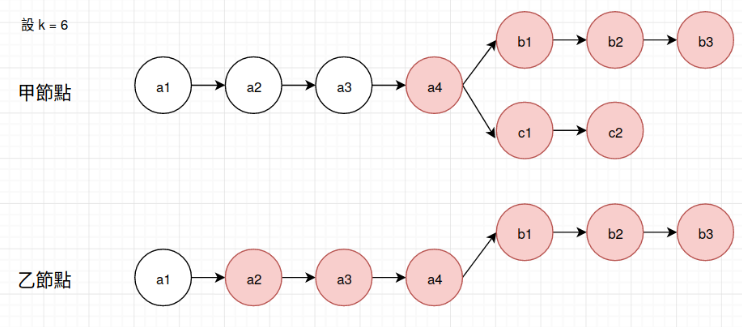
\includegraphics[width=\textwidth]{wrong-cache}
\caption{不一致的快取}
\end{figure}

粉紅色表示在快取,白色區塊則表示不在快取。
此時若有一個不附證明的交易,付款方在 a2 區塊出現過,則乙節點會接收交易,甲節點則不會接收。

\section{快取設計}

一個簡單的設計準則可以避免前述的錯誤:每一個區塊都有自己的快取,
快取的內容僅僅由該區塊所在的鏈的資料所決定。如此,我們把樹狀結構縮減為一個串列,
而不同節點上同個區塊所在的串列必定是相同的,只要每個節點都用同樣的確定性算法從這個串列計算出快取,
就能夠保證每個節點驗證同一個區塊時的快取一致。

\subsection{分叉處理}

觀察以下這條鏈:

\begin{figure}[h!]
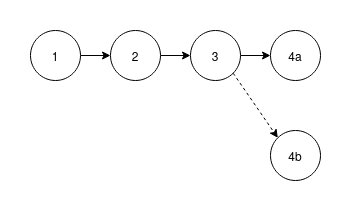
\includegraphics[width=10cm]{快取分叉}
\caption{區塊鏈分叉}
\end{figure}

此時,區塊 4b 嘗試接上區塊 3 ,因此它必須基於區塊 3 的快取來進行驗證。
也就是說,如果我們在接上區塊 4a 時,將區塊 3 的快取直接修改而稱為區塊 4a 的快取,
那當我們要街區塊 4b 時,就無從知悉區塊 3 的快取了,使用某些快取策略時,
我們可以透過回退來取回區塊 3 的快取,但當使用某些快取策略時,遺失的快取無法輕易找回。

即使使用可以回退的快取策略,當分支切換越頻繁,回退的次數也會越頻繁,
而回退的效能可能就會成為瓶頸。

例如在圖 3.3 中,如果同時維持 a, b 兩條分支,則每次接收到非當前分叉的區塊時,都要進行回退,
並且隨着分叉的差異越大,回退的長度也越長,若從 7a 要走到 7b ,就必須先退回 3 ,再走回 7b ,
而事實上若之前曾經從 6a 走到過 6b ,則過程中的大部分運算都是相同的,這顯然是一種浪費。

\begin{figure}[h!]
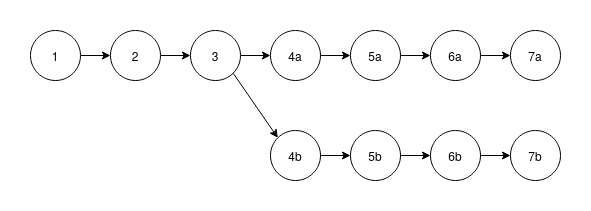
\includegraphics[width=\textwidth]{快取長分叉}
\caption{分叉頻繁切換}
\end{figure}

\subsection{持久化快取}

我們採用另外一種思路:在每個區塊上都保留它自己的快取,當新區塊要接上鏈的時候,
就可以直接取用它前綴區塊的快取,無需重新計算。
換句話說,我們採用全持久化資料結構(fully persistent data structure)~\cite{driscoll1986making}來儲存快取,
每接受一個區塊,就生成一個快取的版本。

在這個方案中,我們必須定時刪除太舊(e.g. 距離最長鏈超過 20 個區塊)區塊的快取,
以將整條鏈的快取大小限制在一定範圍,否則任由快取無限增長將導致記憶體用罄,以致於必須使用到硬碟,
那快取就變得沒有意義了。

這個方案帶來的立即問題是如果我們單純複製前一個區塊的快取,
並基於前一個區塊的快取做修改,那快取的大小將會正比於未刪除的快取的數量。
然而,相鄰區塊中的快取有很高的相似性,若能選用適當的資料結構來讓相鄰區塊共享快取,
將能夠有效提高空間使用率。

\section{快取策略}

不同的快取策略在應對不同工作量(workload)時的命中率各不相同,
以下討論實作簡單的「最近 k 塊」策略,以及實作較為複雜,但經驗上命中率較高的 LRU 策略。

\subsection{最近 k 塊}

在「最近 k 塊」策略中,一個區塊的快取即為由該區塊開始,由高往低取 k 個區塊,
這 k 個區塊中出現過的交易中的資訊。

這本質上就是一種 FIFO (first in first out) 策略,不過是以區塊爲單位。

以下為 k = 6 的示意圖

\begin{figure}[h]
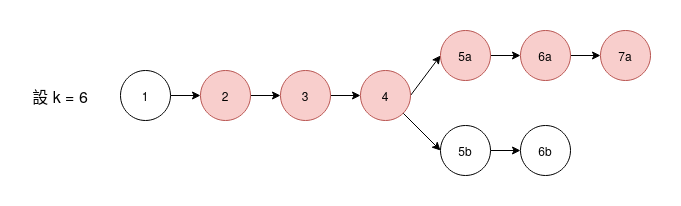
\includegraphics[width=\textwidth]{最近k塊}
\caption{區塊 7a 為粉紅色區塊中的所有交易資訊}
\end{figure}

可以用一個鍵值對(其底層可為雜湊表、搜尋樹、跳錶......等等)來表示快取,
若考慮每次重算的情境,例如在圖 3.4 中,要在 7a 後方額外加入一個 8a 區塊,
則我們加入 8a 區塊中的交易資訊,並丟掉只在 6a 中出現但沒有在其餘區塊中出現的交易資訊。

「最近 k 塊」的快取可以回退,跟前進時的算法一樣,只是換了個方向。

當考慮全持久化,我們可以選用可持久化的鍵值對資料結構,
例如雜湊\cite{bagwell2001ideal}、搜尋樹都有想對應高效成熟的持久化實作,
若一個快取有 n 個鍵,則持久化雜湊/搜尋樹插入/刪除一筆鍵值時,
時間、空間複雜度皆為 $O(log(n))$。

\subsection{LRU}

LRU 是 least recently used 的縮寫,這種策略中,快取大小是固定的,
若快取已滿,在插入新資料之前必須先丟棄一筆資料,
LRU 會去挑選快取中所有資料中最久沒被用到的那一筆來丟棄。

LRU 之所以會被認爲有效,是因爲人們相信,

進一步抽象來看,LRU 是一種支援兩個介面的資料結構,
\begin{itemize}
  \item get(key)
  \item put(key, value)
\end{itemize}

get(key) 時,若 LRU 存在該鍵,則返回對應值,並且將 key 的使用時間調整到最新。

put(key, value) 時,若 LRU 空間未滿,則直接插入一筆鍵值對,
這筆新鍵值對的的使用時間為最新;若 LRU 空間已滿,
就要找出當前快取中使用時間最舊的丟掉,再插入新鍵值對,此新鍵值對的使用時間亦爲最新。

對應到淺狀態區塊鏈的情境中,每當一個區塊要接上,我們要計算新區塊快取時,
會把一系列帳號資訊的讀取跟修改操作轉變成 get 跟 put ,鍵是帳號地址,值是帳號狀態,
然後在 LRU 底層的資料結構上進行相應操作。

當在淺狀態區塊鏈中使用 LRU 策略時,是無法回退的,其原因為 TODO

\section{持久化 LRU 算法}
在討論持久化 LRU 算法之前,我們先觀察如何在軟體上高效實作 LRU 快取,
調查 github 上多個高使用量的 LRU 函式庫,基本不脫以下資料結構:

\begin{figure}[h]
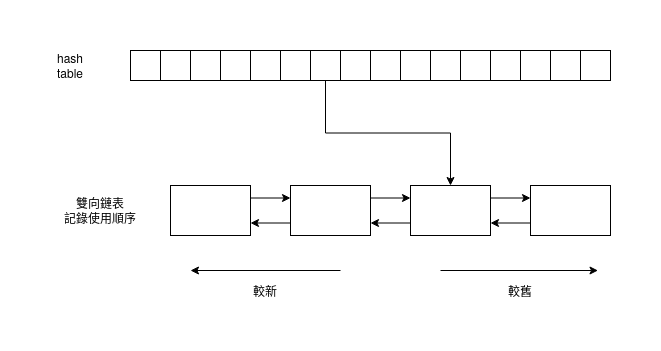
\includegraphics[width=\textwidth]{LRU}
\caption{LRU 資料結構}
\end{figure}

執行 get 時,透過雜湊得到指向值的指針,獲取資料,並且將指針指向的鏈表節點移動至鏈表頭部(最左側)。
執行 put 時,若快取命中,更新節點的值,並將節點移動至鏈表頭部,
若快取未滿,從頭部加入快取值,並將其指針放入雜湊表,
若快取已滿,拔出雙向鏈表的尾部(最右側)節點,並且在雜湊表中移除該舊鍵,
然後在頭部加入快取值,放指針到雜湊表。

觀察到 LRU 需要記錄的資訊有二:

\begin{enumerate}
  \item 由鍵找到值(鍵值對)
  \item 各個鍵的順序資訊
\end{enumerate}

在前述的雜湊表 + 雙向鏈表的實現方案中,雜湊表負責 (1) ,雙向鏈表則負責 (2),
注意到,雙向鏈表極為自然的記錄了順序關係,它甚至不需要記錄確切的擷取時間。

一個簡單的想法是,我們直接把雜湊跟雙向鏈表的持久化替代品組合起來,
就得到了一個持久化 LRU ,然而,雖然持久化雜湊有很成熟的替代品,
持久化雙向鏈表卻沒有很好的替代方案。

因此,我們需要用其他可高效持久化的資料結構來取代雙向鏈表,進一步抽象雙向鍵表做的事情有:

\begin{enumerate}
  \item 更新一個節點的使用時間到最新
  \item 刪除使用時間最舊的節點
  \item 插入新節點,新節點的使用時間爲最新
\end{enumerate}

以下,先討論了如何用紅黑樹\cite{guibas1978dichromatic}(平衡搜尋樹)來完成上述任務,
再介紹我們設計的順序樹資料結構,相比紅黑樹,它能更高效的完成這些任務。

\subsection{雜湊 + 紅黑樹}

\subsubsection{紅黑樹 bulk 優化}

\subsection{雜湊 + 順序樹}